\chapter{Fire prevention}
% COMMENT
\paragraph{} Airport Category nº9:  discharge rate of foam solution/min and water according to foam meeting performance level A.

Fire-Fighters station with two floors linked with vertical slide bars and stairs. 

\begin{description}
	\item[Ground level:] a quick and direct garage for 3 vehicles, plus lockers and depot.
	\item[First floor] with all the facilities such as gym, rest area, bedrooms, washroom, dinning room and infirmary.
\end{description}
% END COMMENT
Central location to guarantee a quick performance.
EXTRA:  Jakarta Fire Extinguisher at 25 km approx.

	\section{Fire prevention regulations }
		\subsection{Level of protection}
		\paragraph{} From ICAO Annex 14 V1, the level of protection at an aerodrome for rescue and firefighting should be equal to aerodrome category determined using the principles in articles \textit{9.2.5} and \textit{9.2.6}.
		
		Table \ref{table91} is used to determine the aerodrome category taking into account the longest aeroplanes normally using the aerodrome.
		
		The biggest plane using the aerodrome is the Boeing 777-300 which have a length of 74m and a fuselage width of 6.2m.
		
		According to this data, the \textbf{Aerodrome category} is \textbf{9}.
		
		\begin{figure}[H]
			\centering
			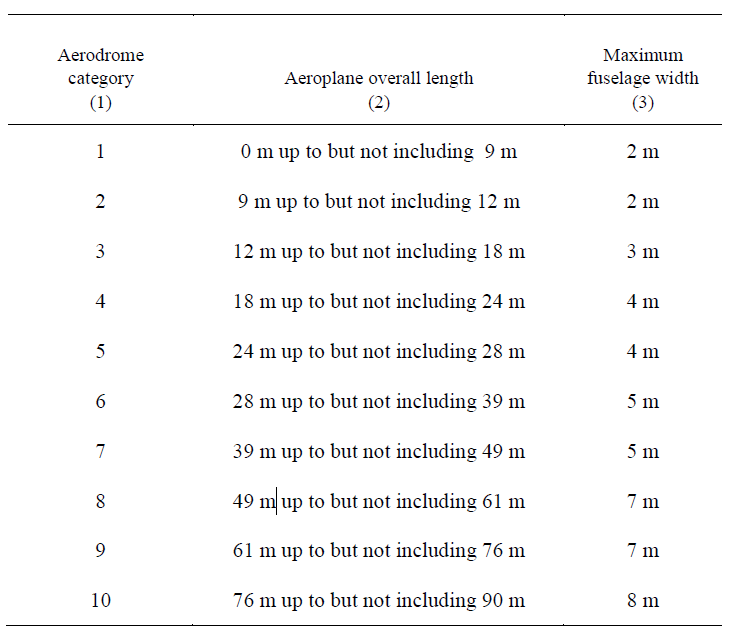
\includegraphics[clip, trim=0cm 0cm 0cm 0cm, width=0.8\textwidth]{./images/firefighting/table91}
			\caption{Aerodrome category for rescue and firefighting.}
			\label{table91}
		\end{figure}
	
		\subsection{Extinguishing agents}
		\paragraph{} Also, from ICAO Annex 14 V1, section 9, the amounts of water for foam production and the complementary agents to be provided on the rescue and firefighting vehicles shall be in accordance with the aerodrome category.
		
		From \textit{Airport Services Manual (Doc 9137), Part 1} and the category of the airport, the level of performance selected is \textbf{level A}. Now the table \ref{table92} can be used to determine the minimum usable amount of extinguishing agents for the airport.  
		\begin{figure}[H]
			\centering
			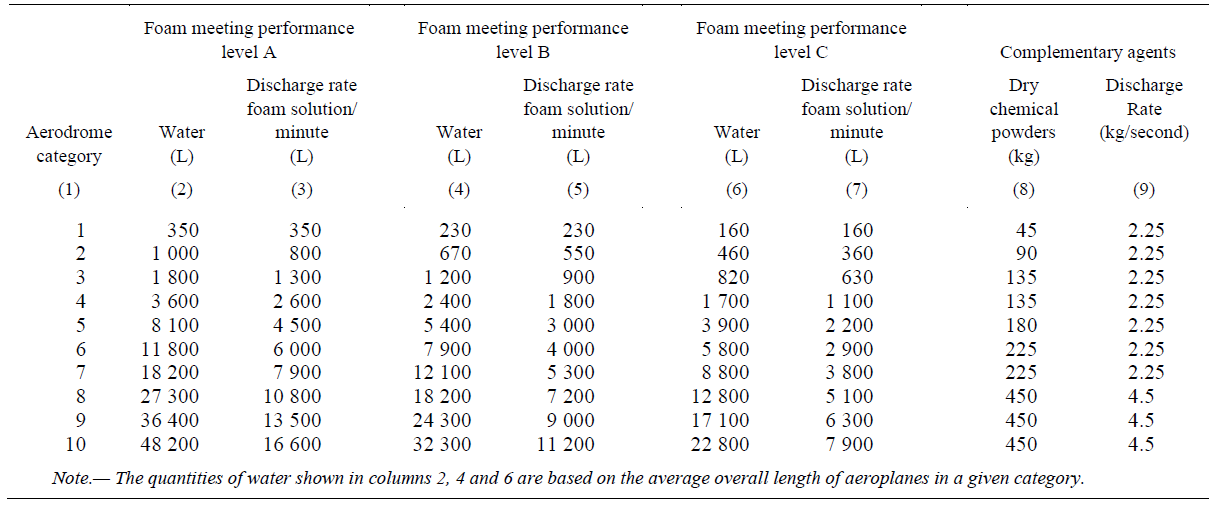
\includegraphics[clip, trim=0cm 0cm 0cm 0cm, width=1\textwidth]{./images/firefighting/table92}
			\caption{Minimum usable amount of extinguishing agents.}
			\label{table92}
		\end{figure}
	
	For a category 9 aerodrome with performance level A, the minimum usable amount of water is 36400 L and 

\section{Chosen materials}
		\subsection{Building elements}
		\subsection{Materials}